% approach.tex
\begin{par}
    \par \hspace{15pt} Inspired by the related reading materials, the group has decided that the generative networks of the project's model should also be a temporal model, which it would have information related to both the entire track and the local segments of the music for pattern recognition. A coarse architecture of the model is demonstrated in Figure \ref{fig:archie}. 

    \begin{figure}[H]
        \centering
        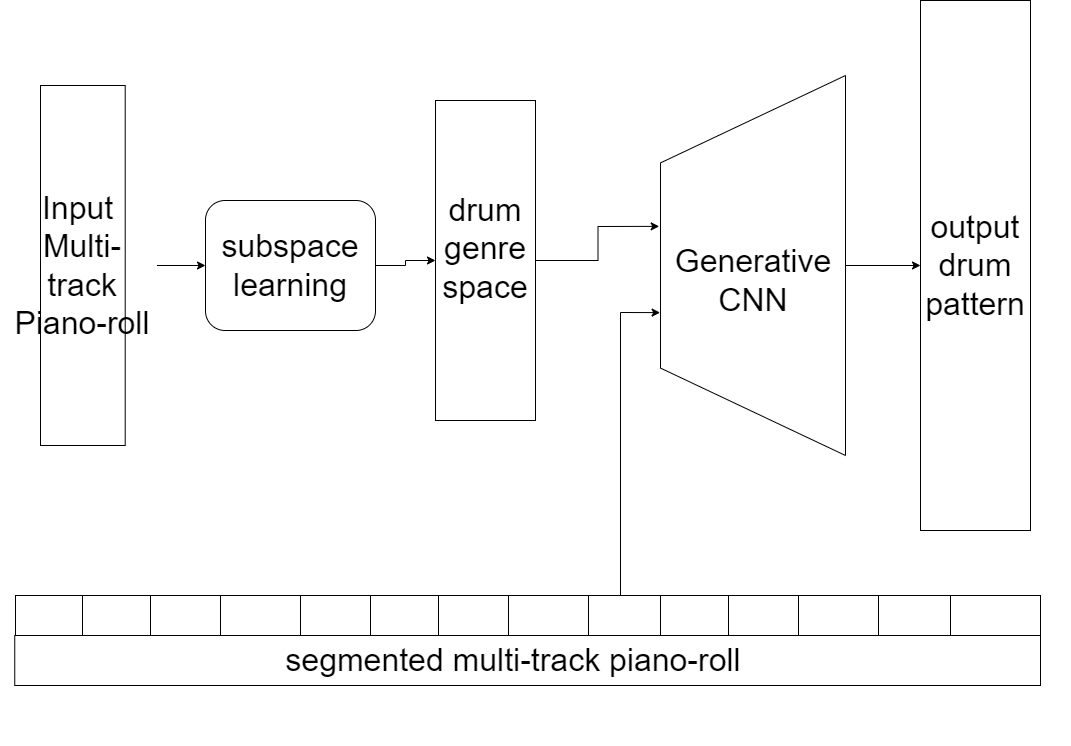
\includegraphics[width=3in]{image/proposal_architecture}
        \caption{Course Architecture of the model}
        \label{fig:archie}
    \end{figure}
    
    \subsection{Pre-Generator Ablations} % (fold)
    \label{sub:Pre-Generator Ablations}
    \par In the above diagram, first the completed tracks of other instruments are collected and feed into a classification/encoding algorithm. The algorithm would produce a drum genre space that will be utilized as the global inductive bias vector $z$ for the segmented generators. The group has proposed three methods for the classification/encoding algorithm to implement this part of the network.

        \subsubsection{CNN Encoders} % (fold)
        \label{ssub:Convolution Neural Network Encoders}
            \par For the first option, the group would like to implement a conventional CNN encoder for the classification/encoding task. It is expected to be the most computationally intensive implementation but the most mature encoding structure available as of today. The group would probably inspect both the CNN encoder with freezed implementation during generation task or continuously fine-tuning the CNN encoder while training for the generation task.

        % subsubsection Convolution Neural Network Encoders (end)

        \subsection{Subspace Learning} % (fold)
        \label{ssub:Subspace Learning}
            \par For the second option, the group would like to test the classification task with the subspaces learning technique. Subspace learning should be much faster in inference comparing to the CNN encoder. \begin{par}
    % Because of the large scale of music data representation, doing training data Dimension Reduction (DR) and Principal Component Analysis(PCA) are essential to a lighter-load training process. Some related works use singular value decomposition(SVD) to find principal components to approximate the structure of the training data \cite{pca}. 
    
    For the music genre classification task of this project, the team currently plans to first group the training data into different music genres, and then use SVD to obtain an orthonormal basis for each genre space. Some related training can be seen in \cite{pca}. After having learned the genre subspaces, classification can be done by comparing the projections of one particular test data onto the orthogonal complement of the genre subspaces.
\end{par}
        % subsection Subspace Learning (end)

        \subsubsection{Perceiver} % (fold)
        \label{ssub:Perceiver}
            \par In the last option, one of the student in the group would like to implement an attention-based model, namely the Perceiver \cite{perceiver}. Since the output space of the perceiver model would be a logits vector, it can also serve as a traditional classifier/encoder structure. This part of the project would potentially be adopted from one of the student's EECS-542, Advanced Computer Vision course project. 
        % subsubsection Perceiver (end)
    % subsection Pre-Generator Ablations (end)

    \subsection{Discriminator Ablations} % (fold)
    \label{sub:Discriminator Ablations}
        \par The group would also like to do a study upon the ablation of the discriminator architecture, which the group also has three variations in mind. 

        \subsubsection{No Discriminator} % (fold)
        \label{ssub:No Discriminator}
            \par The most natural and intuitive idea the group has raised and would like to test on is completely removing the discriminator architecture from the original MuseGAN model.  Thus instead of using a discriminator, the group would like to see if the model would solely work with L2-norm loss between the generated and the labels.
            
        % subsubsection No Discriminator (end)


    % subsection Discriminator Ablations (end)
    
    



\end{par}